\chapter{CCD-based Multispectral Frequency-Domain DOT of Breast Cancer}
\section{Introduction}
Diffuse optical tomography (DOT) of the breast has a long and successful history at Penn where several instruments have been developed to translate DOT techniques to the clinic \cite{corlu_03_1,culver_03_3,Holboke2000,Ntziachristos1999,Ntziachristos2001,Ntziachristos2000,Ntziachristos2002,OLeary1996,Zhu1999}. My work builds on and improves upon these works while addressing some critical limitations the previous generation of the DOT breast imager (Gen2) used in many successful clinical studies \cite{choe_05_1,choe_09_1,corlu_07_1,corlu_03_1,corlu_05_1,culver_03_1}. The new DOT imager (Gen3) includes several feature upgrades: 1) multispectral frequency-domain measurements in the transmission geometry using heterodyne measurement techniques, 2) addition of profilometry systems for enhanced breast segmentation and 3) deployment of the largest clinical source-detector pair datasets for improved 3D reconstructions 4) as well as an improved clinical patient interface. In this chapter, I provide an overview of the Gen3 instrument design and its new features, followed by characterization measurements with tissue simulating phantoms. Finally, clinical results from cancer patients will be shown.

\section{Previous Breast Imaging Device (Gen2)}
The previous DOT imaging device shown in Fig. \ref{fig:gen2pic}. The Gen2 DOT imaging device images the breast in transmission through parallel plate compression geometry. The device illuminates breast tissue with multi-spectral CW light while detecting the transmitted light with a CCD. In addition, the the bulk tissue optical properties is determined using frequency-domain measurements in the remission geometry. The measurement is made with the patient lying prone on a flat bed with her breast inserted inside a recessed box. This box has a grid of source fibers on one side (source plate) with a window on the other (detector plate). The source plate is moved axially to softly compress the breast between the source and detector plates. The box is then filled with a matching fluid with optical properties similar to average human breast tissue before measurement. The matching fluid consists of water, india ink (for absorption) and intralipid (for scattering).
\begin{figure}[ht]
\begin{center}
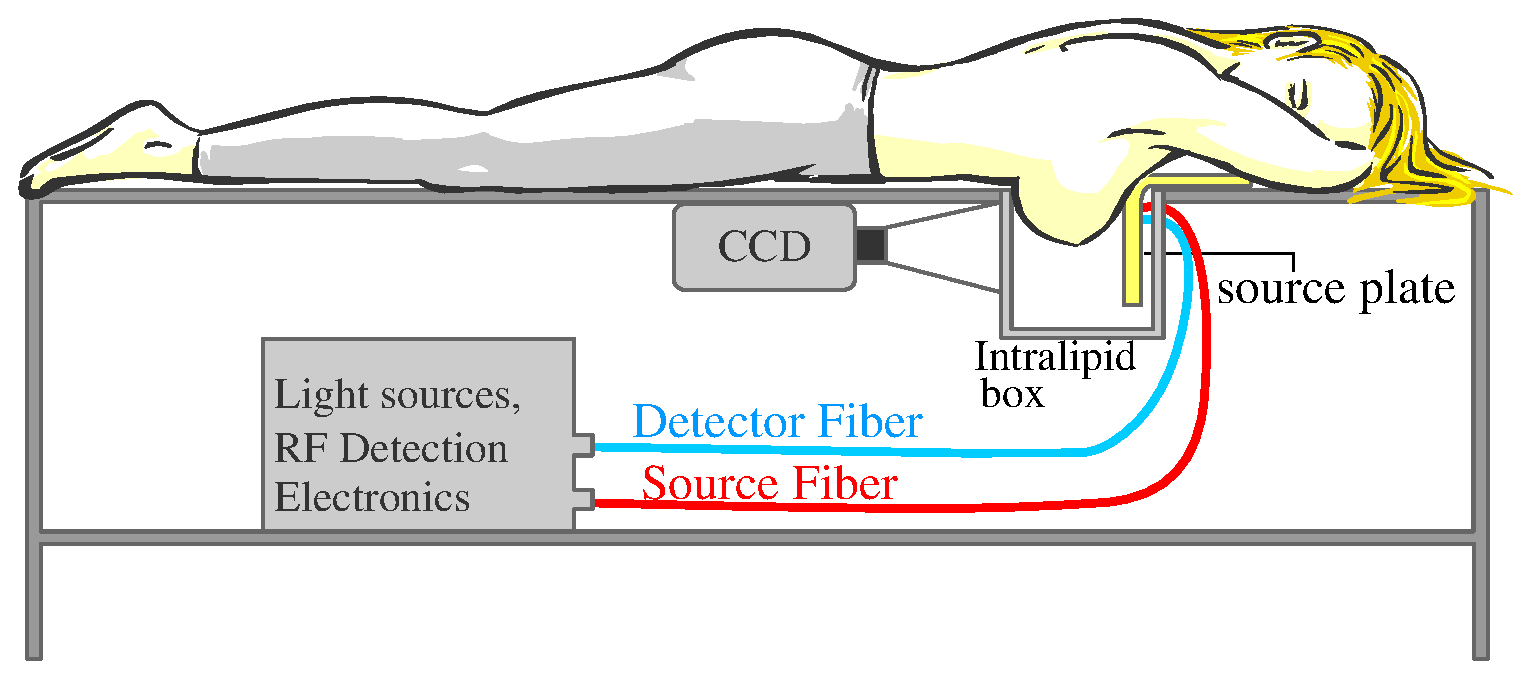
\includegraphics[width=10.5cm]{./figures/4_Gen3/gen2schem.eps}
\caption{Schematic of the previous generation breast scanner.}
\label{fig:gen2schem}
\end{center}
\end{figure}
The source plate has 45 fiber positions arranged in a 9x5 square grid with a spacing of 16 mm between nearest neighbors. The sources are measured in series using cascading optical switches (DiCon Fiber Optics, Richmond, CA). At each source position six measurements are made at varying wavelengths (650, 690, 750, 785, 830, 905 nm) using fiber-coupled laser diodes. On the detection side, a CCD camera (Roper Scientific, Trenton, NJ, VersArray:1300F) collects the light that exits in the transmission geometry focused on the detection window. A image is obtained for for each source and laser combination with an exposure time of 500 ms. From each image a  A 24$\times$41 grid of 984  decimated set is selected from the CCD after 2x2 hardware binning of the pixels. For the frequency-domain remission measurements, four out of the six lasers are modulated at 70MHz. At these wavelengths measurements are made with additional grid of 3mm detector fibers arranged on the source plate in a 3x3 grid with 16 mm spacing. The light from these fibers are collected by an avalanche photodiode for homodyne frequency-domain measurements.

A lot was learned from this device and it informed the design and development of the current DOT breast imager. In general, it is difficult to reduce the cross-talk of absorption and scattering with CW measurements as both can attenuate the level of detected light between a source and detector in a diffuse medium. We showed some success of mitigating this with multi-spectral measurement, but this can be improved upon with frequency-domain measurements. The breast was also compressed in the axial geometry required comparisons of the DOT to MRI images--which are taken in the saggital geometry more difficult.

\section{Clinical Breast Imaging Device (Gen3)}
The Gen3 breast imaging device primarily improves on the previous device through the use of multispectral and frequency-domain illumination and a CCD based heterodyne detection that  improves quantification and separation of absorption and scattering during 3D reconstruction of DOT data. Using a CCD camera for detection allow us to also collect a large number ($10^6$) of source detector pairs in parallel for improved resolution. In addition a supplemental pair of profilometry imaging systems were designed and built (discussed in Sec. \ref{sec:profilometry}) to provide 3D surface information about the breast shape. This 3D breast shape improves segmentation of the reconstruction volume of the breast. Finally, significant effort was made to build a clinical grade device with a patient interface that maximized comfort and minimized movement during our measurement. Software for the device was also developed to enable simple and streamlined operation by our clinical collaborators.
\begin{figure}[ht]
\begin{center}
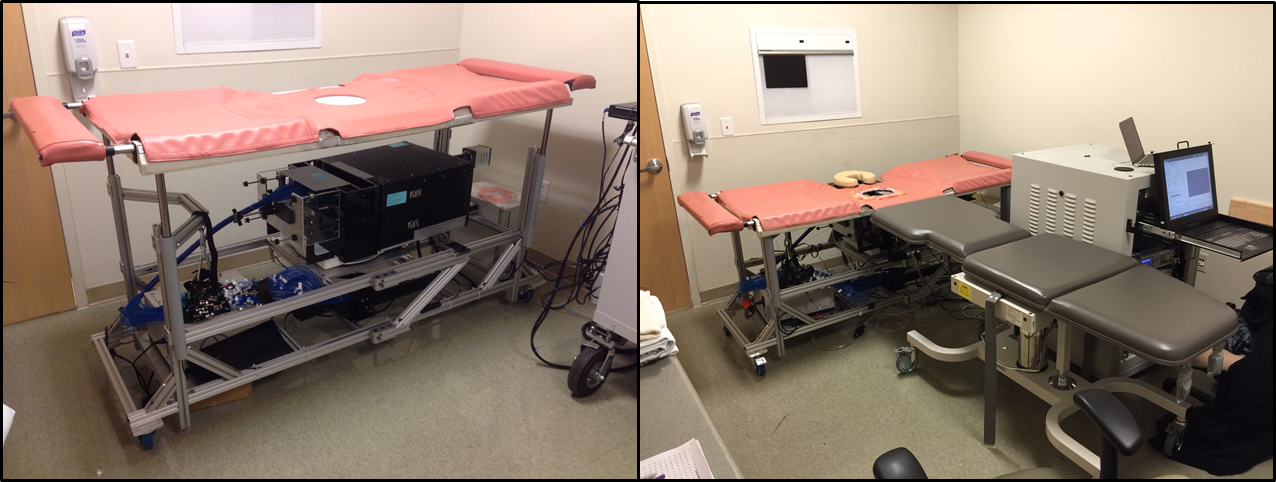
\includegraphics[width=14.5cm]{./figures/4_Gen3/gen3pic3.png}
\caption{Then breast imaging device in the mammography wing of Perelman Center for Advanced Medicine at the University of Pennsylvania (replace later)}
\label{fig:gen3pic}
\end{center}
\end{figure}
\begin{figure}[ht]
\begin{center}
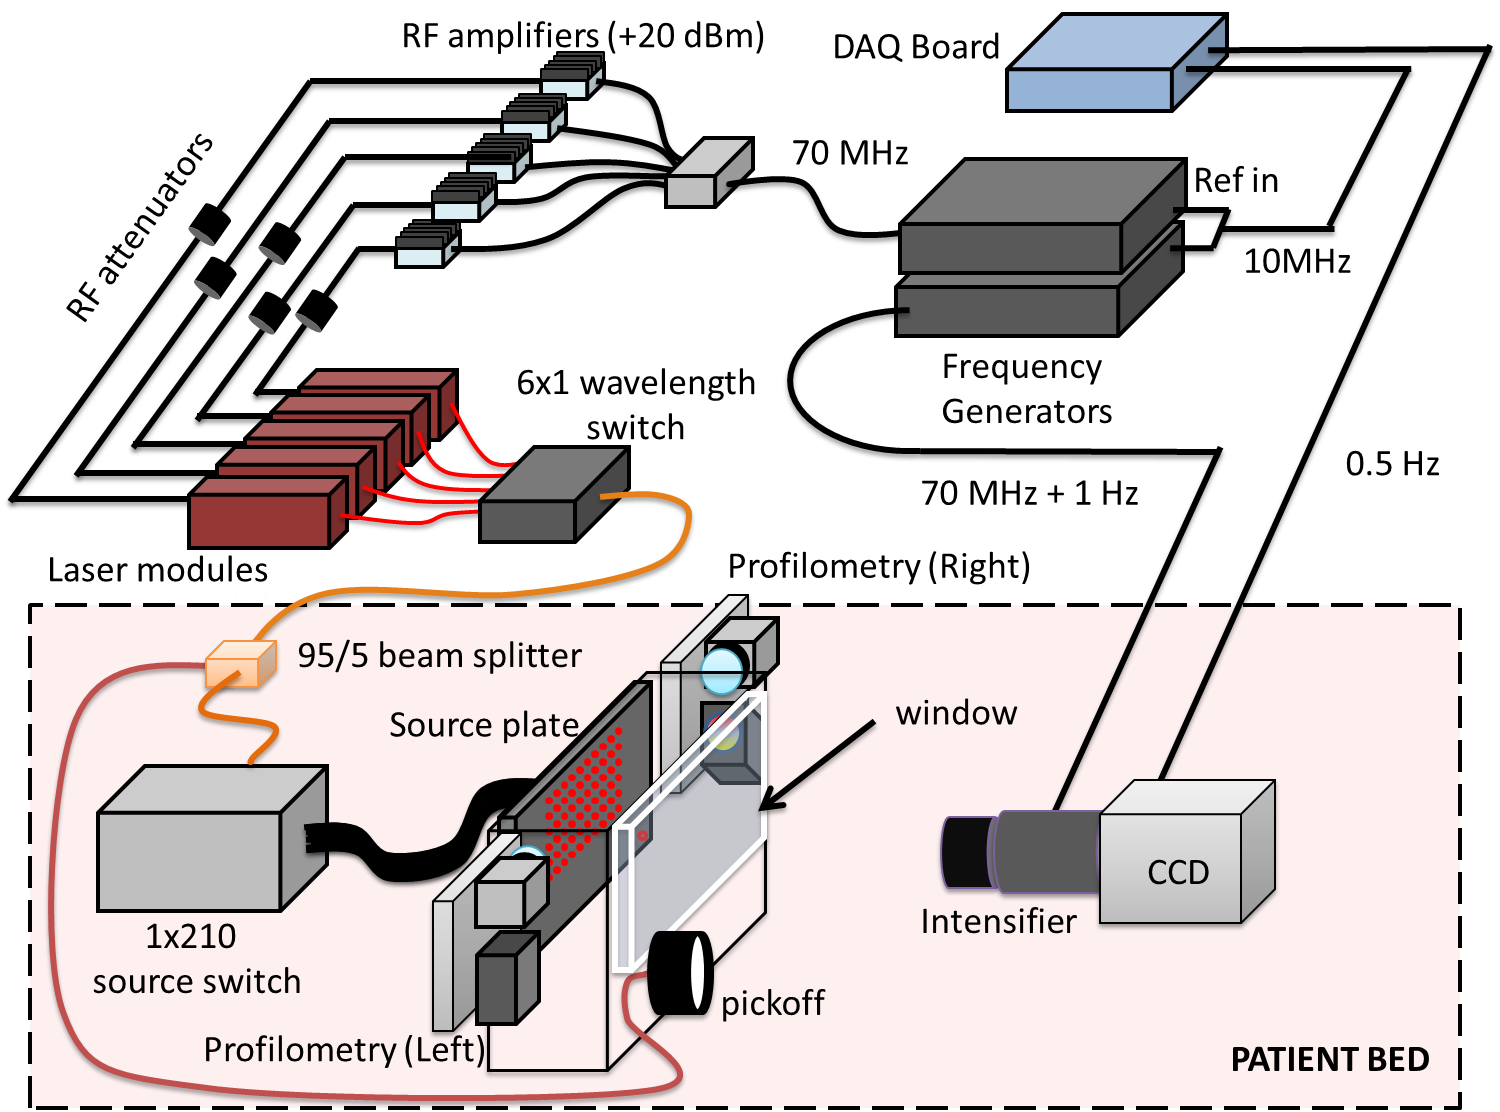
\includegraphics[width=14.5cm]{./figures/4_Gen3/gen3schem.png}
\caption{Schematic of the clinical DOT breast imaging device}
\label{fig:gen3schem}
\end{center}
\end{figure}
The schematic for the clinical breast imaging prototype that I built is shown in Fig.~\ref{fig:gen3schem}. The patient lies prone on a modified biopsy bed while one breast is centered and sagittally compressed between the source plate and window in the breast tank. Typical thickness of compression varies between 56mm and 70mm. The tank is filled with a solution of intralipid and india ink mixture to match the optical properties of tissue of the patient in the NIR wavelength range.

The breast imager comprises of several key components. Briefly, a laser system encompasses optics and electronics for generating frequency-modulated light source at various NIR wavelengths. This light is put through a custom switch to one of 209 source positions inside a breast tank where a breast is inserted. The breast tank has two sets of profilometry cameras and projectors for 3D segmentation. Lastly, we have a gain-modulated detection using an image intensifer mounted CCD. I wil now discuss each of these subsystems in detail in the following sections.

\subsection{Laser System}
Illumination is provided by laser diodes with the wavelength of $660$, $690$, $785$, $808$, and $830\,{\rm nm}$ . Table \ref{fig:lasertable} provides detailed characteristics of each laser module (Fig.~\ref{fig:laserpic}). The laser diodes are mounted on a custom copper block for a TEC cooler and cooled to $-13^{\circ}{\rm C}$. Each laser diode is driven and temperature controlled by a dedicated ILX mainframe module (instrument info). The lasers are amplitude modulated at $70\,{\rm MHz}$ using a an RF signal from a frequency generator (Rhode and Schwartz, SMB100). More specifically, the $70\,{\rm MHz}$ RF signal from the frequency generator is combined with the DC current from the ILX driver for each laser with ??? (minicircuit). The DC and RF voltage input for each laser was optimized using RF amplifiers (?), RF attenuators (?). The laser driver current is optimized for the best modulation depth ($>80 \%$) and a sinusoidal waveform. The frequency modulated light from each fiber coupled laser is then coupled to a 6x1 100 $\mu m$ core optical switch (Optojenna) which allows the system to switch wavelengths in series.
\begin{figure}[ht]
\begin{center}
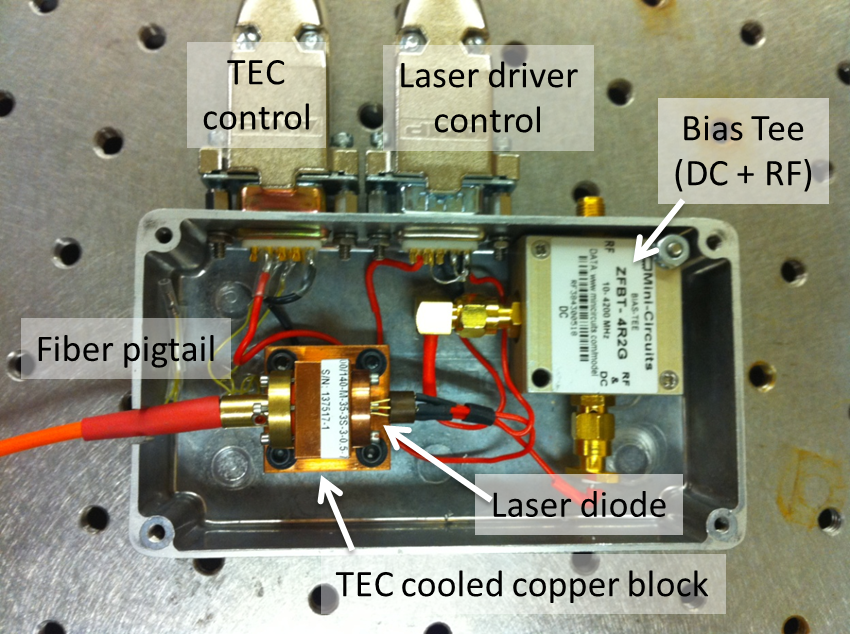
\includegraphics[width=10cm]{./figures/4_Gen3/laserpic.png}
\caption{Schematic of the clinical DOT breast imaging device}
\label{fig:laserpic}
\end{center}
\end{figure}

\subsection{Source Position Switch and Source Plate}
The output fiber from wavelength switch is connected in series to a $95/5$ fiber beam splitter with the $5\%$ going to the the pickoff--to be discussed in Sec. \ref{sec:datanorm}--and $95\5$ going to a custom 1x210 channel optical galvo switch. Switching through 210 channels with a conventional cascade of switches used in the previous system based on mechanical or prism switch mechanisms is costly, slow, and have high throughput losses. The custom switch collimates light from a $100\,\mu{\rm m}$ input fiber and uses galvo controlled mirrors to direct the light into a telecentri lens which then focuses the light onto a bundle with 210 $600\,\mu{\rm m}$ core fibers as shown in Fig \ref{fig:BundleFace.jpg}. Each fiber is connected to a custom hand-polished patch fiber with a metal ferrule tip that connects to the source plate. 209 of the source fibers are arranged in a 11x19 square grid with 8 mm spacing on each side on a black delrin plate. The source plate is moved against the detection window and a picture is taken to determine source positions for reconstruction as shown in Fig \ref{fig:srcplatepic} One of the remaining fiber is used as a calibration source placed far away from the source grid. The purpose of this calibration source will be discussed in Sec. \ref{sec:datanorm}.

%\begin{figure}[t]
%\centering\includegraphics[width=7cm]{./figures/GalvoPic.png}
%\caption{\label{fig:GalvoSwitchPic}
%  Photograph of the (a) galvo switch and the (b) input face of the fiber bundle (c) custom patch cable (d) source plate
%\end{figure}

\begin{figure}[ht]
\begin{center}
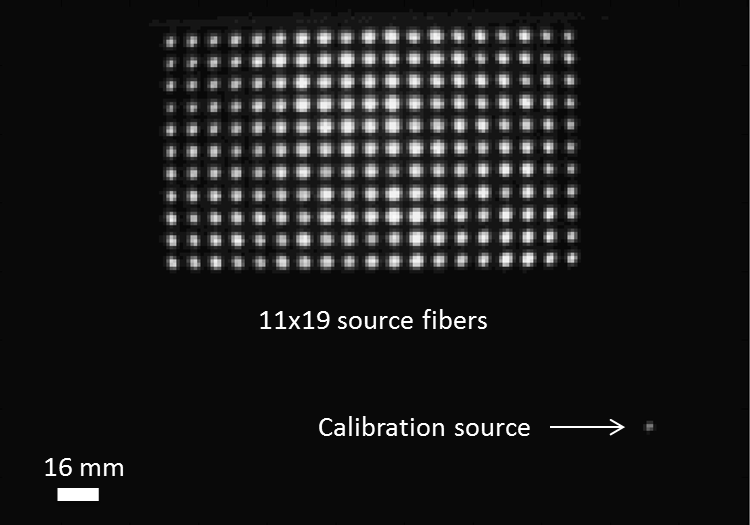
\includegraphics[width=10.5cm]{./figures/4_Gen3/srcplatepic2.png}
\caption{Source plate picture taken by Breast Imager CCD after it has been moved up to the detection window. The fibers are backlit by illuminating the back of the fiber bundle. This picture is used to determine the source position for reconstructions.}
\label{fig:srcplatepic}
\end{center}
\end{figure}


\subsection{Breast Tank and Patient Bed}
The breast imaging system is built around a modified biopsy patient bed. The bed allows for more of the breast to be inserted into the tank for greater breast coverage. The breast tank is located right below the hole in the biopsy patient bed. The tank consists a tank with a rail mounted source plate made out of black delrin to maintain parallel compression between the source plate and window. On the opposite side is an acrylic window with anti-reflective coating. The space between the window and the detection setup is covered by a light box that prevents stray signal from reaching the image intensifier and CCD. The tank is also mounted on ball-bearing surface which allows the breast tank, light box, and detection system to rotate 90 degrees for either sagittal or axial compression of the breast.

%\begin{figure}[t]
%\centering\includegraphics[width=7cm]{./figures/BiopsyBedPic.png}
%\caption{\label{fig:BiopsyBedPic}
%  Photograph of the (a) galvo switch and the (b) input face of the fiber bundle
%\end{figure}

\subsection{Image Intensifier mounted CCD}
The detection system consists of a back-illuminated EMCCD (Andor iXon DV887, Ireland) with quantum efficiency optimized in the $500-700\,{\rm nm}$ range. One of the most attractive features of this CCD was its "frame transfer" function which allows for shutterless continous measurement which would be beneficial for our heterodyne measurement scheme in Sec. \ref{sec:heterodyne}. This CCD is mounted with a gain-modulated image intensifier (Lambert Instruments, II8MD GENIII, Netherlands) with a P43 Phosphor screen with a peak emission at $545\, {\rm nm}$. The lens element in front of the image intensifier is a Xenon $25\,{\rm mm}$ $f/0.95$ C-Mount Lens for 1-Inch CCD (Schneider Optics, Germany). The $512 \times 512$ pixel CCD is cropped to a field of view of the breast tank window with a $2 \times 2$ hardware binning for an image $155 \times 200$ pixels with a dpixel of $0.33\, {\rm mm/pixel}$ with a 16-bit depth. The gain on the image intensifier is modulated at  $70\,{\rm MHz} + 1 {\rm Hz}$

\subsection{Frequency-Domain Heterodyne detection}
\label{sec:heterodyne}
The primary goal of the DOT system is to measure the amplitude attenuation and phase shift of the input light as it transits through the breast tissue. There are two approaches to demodulate a high frequency RF signal to estimate $\delta A$ and $\delta phi$: homodyne and heterodyne. Homodyne systems have been developed for optical imaging \cite{Troy1996,Sevick-Muraca1997,Godavarty2003}, but here we describe the heterodyne approach.

Our system uses the well known optical heterodyne detection scheme [cite] where the input signal $\omega_{s}$ is nonlinearly mixed with a reference signal at the same frequency which is offset by a small cross correlation frequency $\omega_{cc}$ such that $\omega_{g}=\omega_{s}+\omega_{cc}$ and the resulting beat frequency at $\omega_{cc}$ is measured.  In our system, $\omega_{s}$ and  $\omega_{g}$ are produced by a pair of phase-locked frequency generators. The lasers in the devices are modulated at $\omega_{s}=70\,{\rm MHz}$ such that the light source intensity can be described as
\begin{equation}
I(t) = I_{0} + I_{\omega}\cos(\omega_s t+\phi_I)
\end{equation}
where  $I_{0}$ is the DC amplitude, $I_{\omega}$ the AC amplitude and $\phi_I$ is the phase offset of the laser. When the light passes through our breast tank diffusively through breast or intralipid solution the resulting transmitted light has the form
\begin{equation}
T(t) = I_{0}A_{DC}({\bf r}) + I_{\omega}A_{AC}\cos(\omega_s t +\phi_I+ \phi({\bf r}))
\end{equation}
where $A_0$, $A_{AC}$, and $\phi$ are the spatially varying DC, AC, and phase information that we are measuring from the surface of our diffusive breast or intralipid solution. On the detection side, we modulate the gain of the image intensifier at $\omega_{g}=70\,{\rm MHz} + 1 {\rm Hz}$ so that the image intensifier sensitivity is
\begin{equation}
G(t) = G_{0} +G_{\omega} \cos((\omega_s+\omega_{cc})t+\phi_G))
\end{equation}
\noindent
where $G_{0}$ is the DC amplitude, $G_{\omega}$ the AC amplitude and $\phi_G$ is the phase offset of the image intensifier gain. The signal that is detected by the CCD after the image intensifier is then
\begin{equation}
S = I(t) \times G(t) = (I_{0} + I_{\omega}\cos(\omega_s t+\phi_I))(G_{0} +G_{\omega}\cos((\omega_s+\omega_{cc})t+\phi_G)).
\label{4_signal}
\end{equation}
The CCD measures the light intensity out of the image intensifer at rate of $10\, {\rm frames/s}$ with frame transfer mode with an exposure time $\sim100\, {\rm ms}$ which in addition to the phosphor screen response time of the image intensifier of $\sim{\rm ms}$ acts as a low pass filter on the signal. Thus (Eqn \ref{4_signal}) simplifies to
\begin{equation}
\label{eqn:heterodyne}
S  = I_{0}G_{0}A_{DC}({\bf r}) + I_{\omega}G_{\omega}A_{AC}\cos(\omega_{cc}t+\phi_I-\phi_G+\phi({\bf r})).
\end{equation}
where we are able to measure $I_{0}G_{0}A_{DC},\,I_{\omega}G_{\omega}A_{AC}$ and $\phi_I-\phi_G+\phi$ for each CCD pixel.

\subsection{DOT measurement and timing}
The measurement timing is controlled using a National Instruments DAQ board (serial) which has an onboard clock as well as analog and digital I/O which can be programmed via Labview software on a computer. The DAQ board is programmed to put out two syncronized clocked TTL signals at $10\,{\rm MHz}$ and $0.5\,{\rm Hz}$. The $10\,{\rm MHz}$ goes to the reference input of the two frequency generators to phase lock the two together. The 0.5Hz signal is sent to the CCD to trigger the beginning of the 17 sequential measurement series synchronizing to the heterodyne measurement via the frequency generators.

In our measurement protocol we switch through all the source positions for each wavelength in series. The measurement at each source position is two seconds long (each triggered by the $0.5\,{\rm Hz}$ signal) resulting in a total measurement time per scan of $2\,{\rm s} \times 209\,{\rm sources} \times 5$ wavelengths $\sim 35$ minutes. For each two second measurement, 17 exposures are captured at at $10\,{\rm frames/s}$ for a total of $1.7\,s$. The remaining $300 {\rm ms}$ is used to write data from the camera buffer to the computer harddrive and switch to the next source position and/or wavelength. To get the $I_{0}G_{0}A_{DC},\,I_{\omega}G_{\omega}A_{AC}$ and $\phi_I-\phi_G+\phi$ from the heterodyne measurement mentioned in Sec. \ref{sec:heterodyne}, the time series (over 17 frames) light intensity for each pixel is fit to Eqn. \ref{eqn:heterodyne} fitted for these variables as shown in Fig. \ref{fig:timeseries}. 
\begin{figure}[ht]
\begin{center}
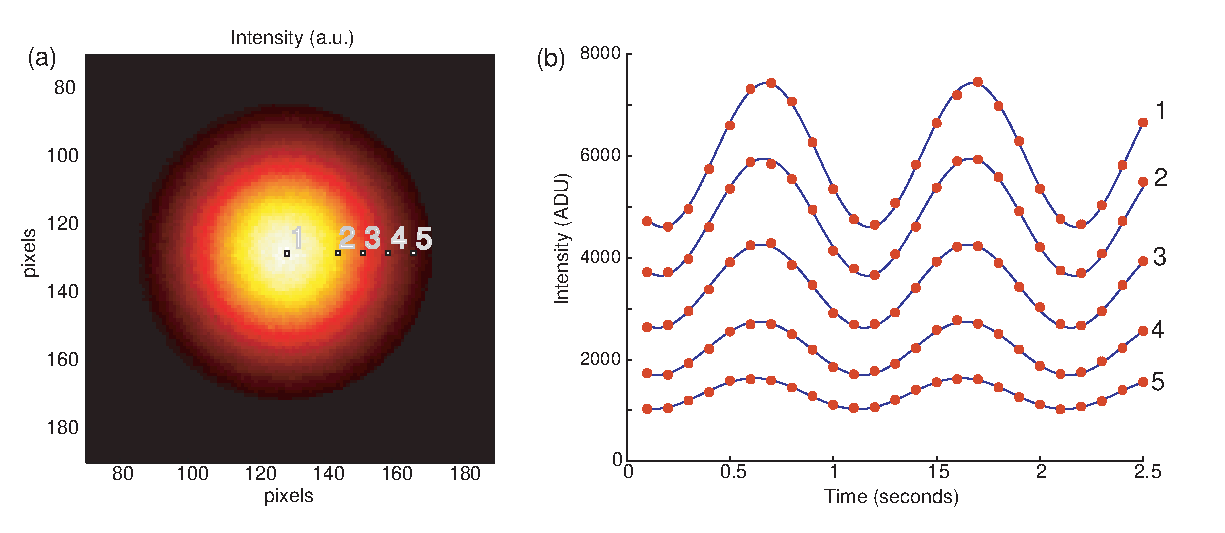
\includegraphics[width=14.5cm]{./figures/4_Gen3/timeseries.eps}
\caption{a) single time frame of light measured by the CCD. b) light intensities for pixels over time. This data is fit for DC, A, and $\phi$.}
\label{fig:timeseries}
\end{center}
\end{figure}

\section{Data Normalization}
\label{sec:datanorm}
A single breast scan will allow us to determine $I_{0}G_{0}A_{DC},\,I_{\omega}G_{\omega}A_{AC}$ and $\phi_I-\phi_G+\phi$ as we saw in Sec. \ref{sec:heterodyne}. However, the quantities that we are interested in are $A_{DC},\,A_{AC}$ and $\phi$ due to the optical properties of the breast. By taking a second reference scan with just the intralipid solution, we can divide out $I_{0}G_{0},\,I_{\omega}G_{\omega}$ and subtract out $\phi_I-\phi_G$.

In addition, we use a pickoff channel shown in Fig \ref{fig:gen3schem} to correct for any changes in amplitude or phase due to laser or RF instabilities before the galvo switch. 5 percent of the light is diverted using a 95/5 optical beam splitter and the fiber is run in front of the window with a 1-inch thick white delrin placed in front of the fiber tip used as a diffuser as shown in Fig \ref{fig:pickoffpic.jpg}. Because it is placed in the FOV of the window, this measurement is taken concurrently with each source measurement. An attenuator has been added to the pickoff so that the light level will be appropriate for the gain and dynamic range of the DOT measurement. 

Finally, we have one additional source of normalization that is used. The device has one additional source channel from the galvo switch which is placed very far from where the breast will be measured as shown in Fig \ref{fig:srcplatepic}. We call this the calibration source. Since it is just another source position fiber, this measurement is not taken concurrently, but rather in series with the DOT measurements. The calibration measurement is typically taken after every 10 sources. The advantage of this source is that is that unlike the pickoff, the calibration source corrects for the galvo and the reference tank and is useful for correcting long-term drifts in the system.

\section{Profilometry}
\label{sec:profilometry}
\subsection{Basics of Profilometry}
\begin{figure}[ht]
\begin{center}
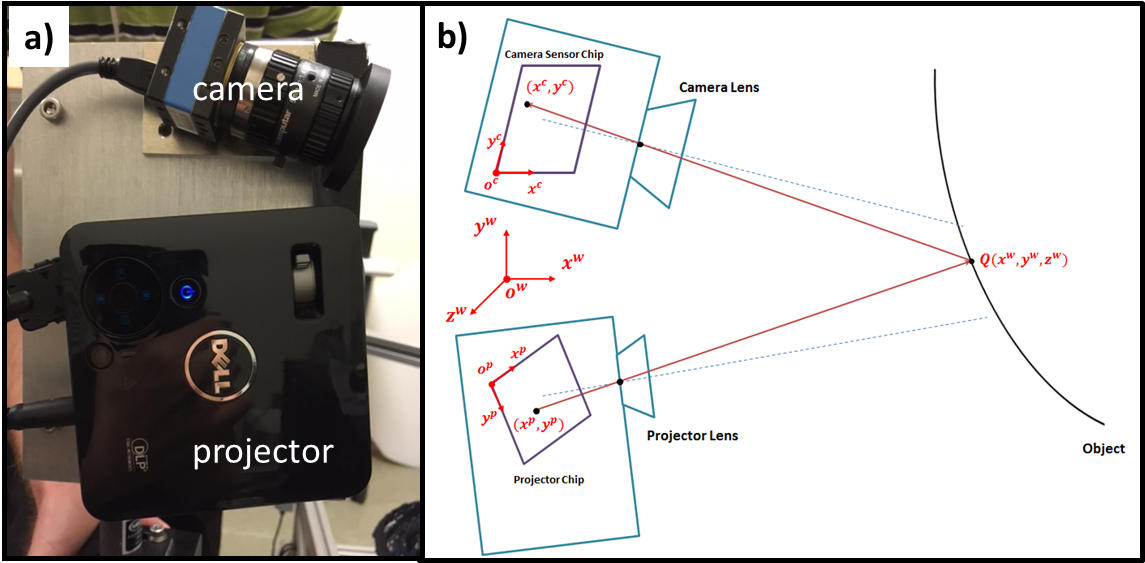
\includegraphics[width=14.5cm]{./figures/4_Gen3/profcoord.png}
\caption{a) Profilometry setup which consist of a ccd camera and a portable projector. b)the schematic with the coordinate systems for the camera, projector, and the world or object coordinate.}
\label{fig:profcoord}
\end{center}
\end{figure}
To improve our reconstruction quality, we have built two sets of imaging devices based on fringe projection profilometry technique. A review on various implementation of this technique can be found in \cite{}. We chose to implement the techniques proposed by Zhang et. al \cite{Zhang2006} with an emphasis on speed, reduced dependance on a need for projector gamma calibrations (which are time consuming). 
Fig. \ref{fig:profcoord} shows the picture of the profilometry device and the corresponding schematic with the related coordinate systems for the camera, projector, and the world or object coordinate. The basic principle of fringe projection profilometry is to project fringe patterns onto an object and to map the phase shift of the patterns to the object height. To accomplish this, one must calibrate the profilometry device to determine the spatial transform function between the camera, projector, and object coordinates. Then a calibration to determine the one-to-one function between the phase shift and object height. The calibration methods for this is detailed in the following references \cite{Peng2007,Zhang2010,Gorthi2010,Geng2011}.

Once the calibrations are set, obtaining the 3D surface profile of an object (in our case the breast surface) requires three steps: 1) projecting fringe patterns onto the object and measure the fringe distortions (Eqn. \ref{eqn:fringe}, 2) convert the distorted images into a phase map, and 3) unwrapping the phase as the phase map is limited to [$-\pi, \pi$].
\noindent
{\bf Step 1:} Project fringe patterns with the following equations:
\begin{eqnarray}
\label{eqn:fringe}
I_{c,1}(x_c,y_c) & = & I_{c,dc}(x_c,y_c)+I_{c,ac}(x_c,y_c)\cos(\phi_c(x_c,y_c)-2\pi/3)\nonumber \\
I_{c,2}(x_c,y_c) & = & I_{c,dc}(x_c,y_c)+I_{c,ac}(x_c,y_c)\cos(\phi_c(x_c,y_c))\nonumber\\
I_{c,3}(x_c,y_c) & = & I_{c,dc}(x_c,y_c)+I_{c,ac}(x_c,y_c)\cos(\phi_c(x_c,y_c)+2\pi/3)
\end{eqnarray}
\noindent
where $I_{c,dc}$ is the average intensity, $I_{c,dc}$ is the modulation amplitude and $\phi_c$ is the phase value to be solved to extract our high information. The subscript $c$ denotes that this is in the camera reference.
\noindent
{\bf Step 2:} convert into phase map by solving for $\phi_c$ using Eqn. \ref{eqn:fringe} which gives us
\begin{equation}
\phi_c(x_c,y_c)=\arctan\big(\frac{\sqrt{3}(I_{c,1}(x_c,y_c)-I_{c,3}(x_c,y_c)}{2I_{c,2}(x_c,y_c)-I_{c,3}(x_c,y_c)}\big).
\end{equation}
\noindent
{\bf Step 3:} Unwrap $\phi_c$ to get the unwrapped phase
\begin{equation}
\Phi_c(x_c,y_c)= \phi_c(x_c,y_c)+2\pi\cdot k(x_c,y_c)
\end{equation}
where $k$ is found by projecting an additional set of images on the object to encode binary information in the image as proposed by Zhang et. al \cite{Zhang2006}. The schematic diagram of the projections used and the binary encoding method is shown in Fig \ref{fig:profunwrap}. Implementing these steps, we are able to unwrap the phase in the steps are shown in Fig \ref{fig:proffringe}.
\begin{figure}[ht]
\begin{center}
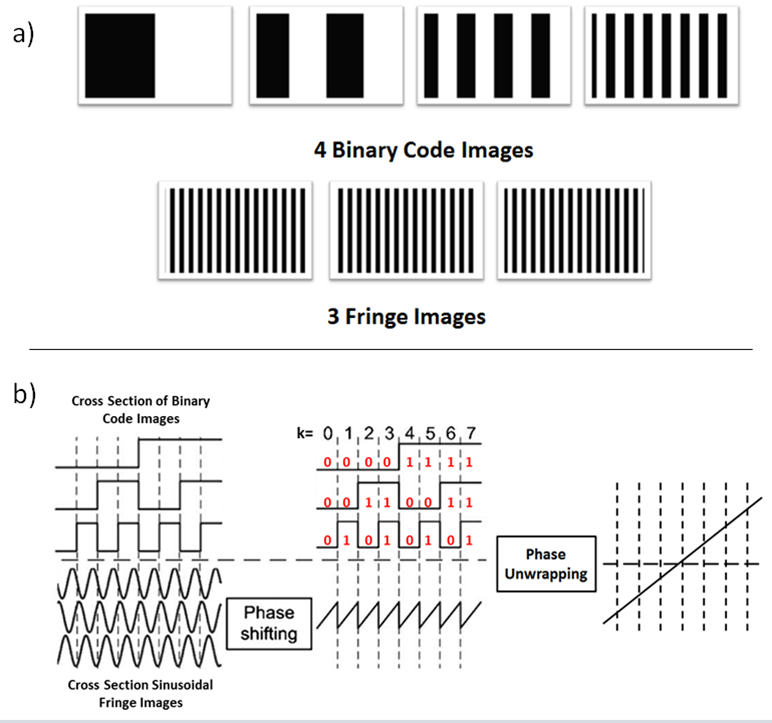
\includegraphics[width=14cm]{./figures/4_Gen3/profunwrap.png}
\caption{a) binary and fringe projections from the projector. b) unwrapping scheme proposed by Zhang et al. using the binary information encoded by the binary projections.}
\label{fig:profunwrap}
\end{center}
\end{figure}
\begin{figure}[ht]
\begin{center}
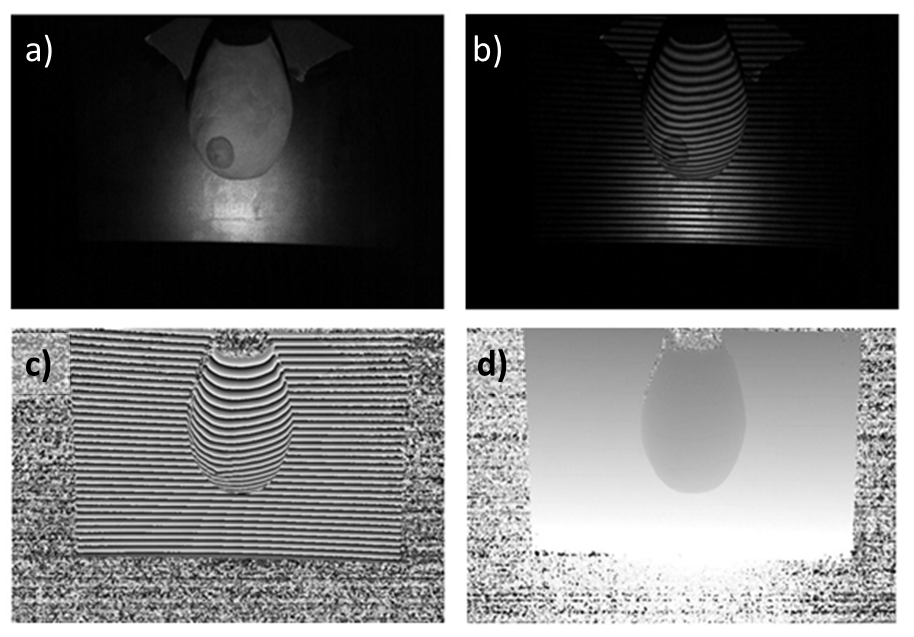
\includegraphics[width=14cm]{./figures/4_Gen3/proffringe.png}
\caption{a) object image b) fringe patterns projected onto object c) phase image d) unwrapped phase image.}
\label{fig:proffringe}
\end{center}
\end{figure}

\subsection{Profilometry for DOT segmentation}
The pair of profilometry devices we built are mounted on the DOT breast imager as show in Fig \ref{fig:proftank}. Fig \ref{fig:profdata} shows data from a human subject. Fringe pattern data is collected from each of the two profilometry devices as well as a sagittal image from the CCD where the outer edge has been traced by hand with a red line. The two surface point cloud generated by the profilometry phase map is combined with the outer trace (red line) of the breast image from the CCD to generate a 3D surface fit to generate a surface on the bottom side of the breast that was not illuminated by the profilometry projectors. This 3D surface fit is then used to generate a tetrahedral mesh to be used in the DOT image reconstruction.

\begin{figure}[ht]
\begin{center}
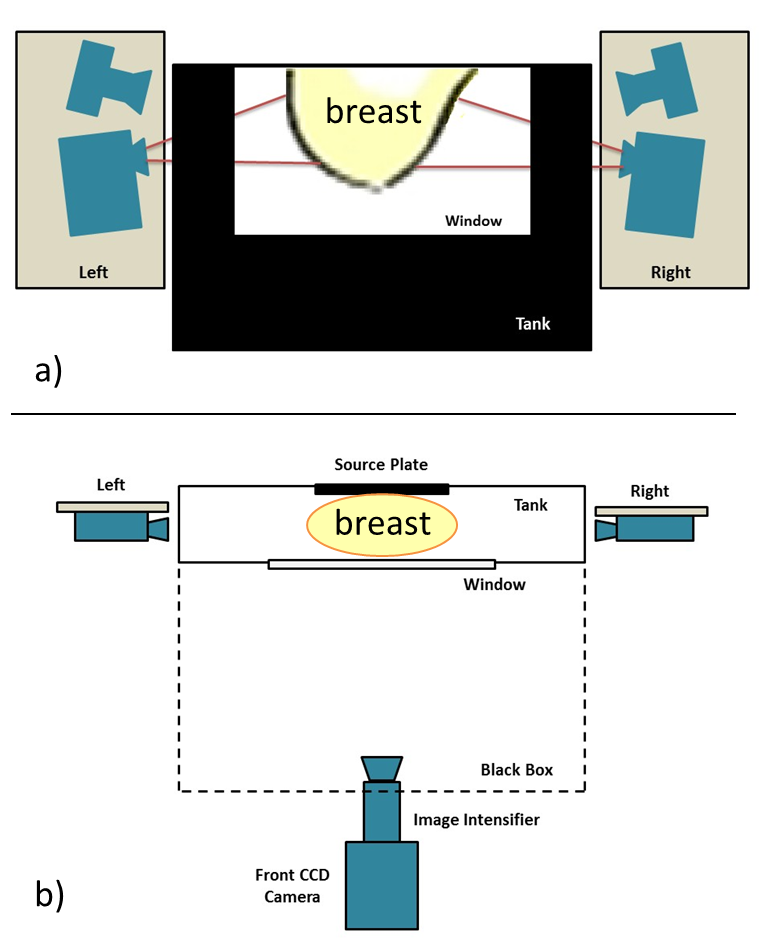
\includegraphics[width=12cm]{./figures/4_Gen3/proftank.png}
\caption{a) Front view of profilometry system with respect to Gen3 breast tank from perspective front CCD camera b) top view}
\label{fig:proftank}
\end{center}
\end{figure}
\begin{figure}[ht]
\begin{center}
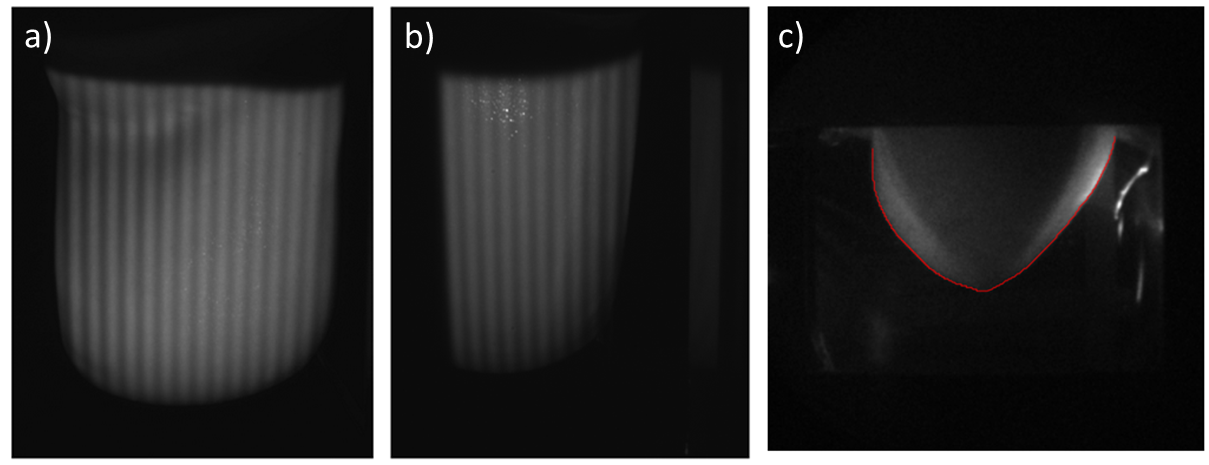
\includegraphics[width=12cm]{./figures/4_Gen3/profdata.png}
\caption{ a) fringe pattern projected on the breast (left side of tank) b) fringe pattern on right side of tank c) sagittal view of breast from front CCD. Red line shows outer edge of breast traced by hand.}
\label{fig:profdata}
\end{center}
\end{figure}
\begin{figure}[ht]
\begin{center}
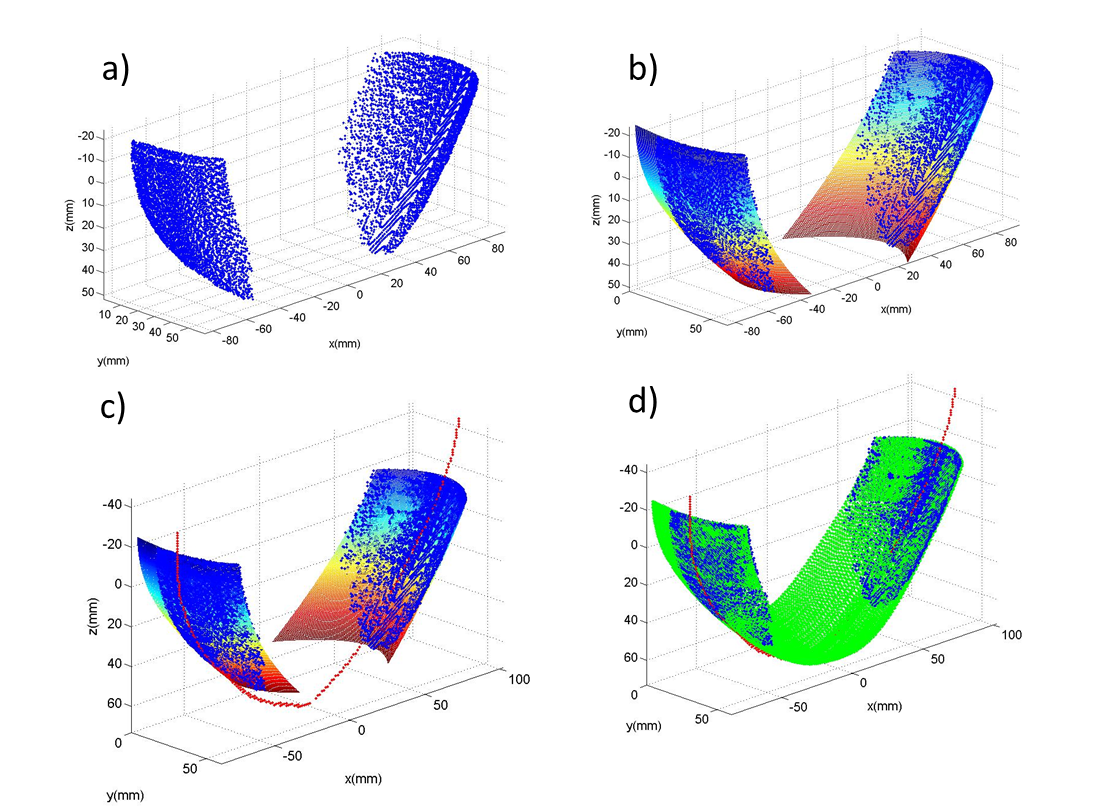
\includegraphics[width=14.5cm]{./figures/4_Gen3/proffit.png}
\caption{ a) 3D point cloud generated by fringe profilometry b)  surface fit of 3D point cloud c) line trace (red) from front CCD camera scaled and translated to match side surfaces d) 3D surface fit of whole breast generated from fringe profilometry data and front image trace.}
\label{fig:proffit}
\end{center}
\end{figure}

\section{Device characterization and testing}

\section{Clinical Results}